\documentclass[10pt, compress, usenames, dvipsnames]{beamer}
\usetheme[progressbar=frametitle]{metropolis}

\usetheme[progressbar=frametitle]{metropolis}
\usepackage{appendixnumberbeamer}

\usepackage{booktabs}
\usepackage[scale=2]{ccicons}

\usepackage{pgfplots}
\usepackage[dvipsnames]{xcolor}

\usepgfplotslibrary{dateplot}

\usepackage{xspace}
\newcommand{\themename}{\textbf{\textsc{metropolis}}\xspace}
\usepackage[langlinenos]{minted}

\usepgfplotslibrary{dateplot}

\usemintedstyle{trac}


\setbeamercolor{framesubtitle}{fg=mDarkTeal}
\addtobeamertemplate{frametitle}{}{%
  \ifx\insertframesubtitle\@empty\else%
  \usebeamerfont{framesubtitle}%
  \usebeamercolor[fg]{framesubtitle}%
  \insertframesubtitle%
  \fi%
}

\title{FShark}
\titlegraphic{\hfill
  \includegraphics[height=.3\textheight]{fsharklogo.png}}
\subtitle{Effortless GPU Programming in F\#}
\author{Mikkel Storgaard Knudsen}
\institute{Master's Thesis presentation, University of Copenhagen}

\begin{document}

\maketitle

\begin{frame}[fragile]
\frametitle{What's the deal?}
\pause
\begin{itemize}
\item<+-> The future demands more efficient computing
\item<+-> not achievable by common sequential programming 
\end{itemize}
\pause 

% CUDA and OpenCL exists, but is a nuisance to write, and to use in mainstream languages

% we want a way to both develop and use efficient GPU computational kernels
% within mainstream language contexts.

\end{frame}

\begin{frame}[fragile]
\frametitle{Bird's eye view - A C\# Code Generator}
  
\begin{columns}[T] % align columns
\begin{column}{.48\textwidth}
  {\scriptsize
  \begin{align*}
    A &=& \begin{bmatrix}
      1 & 2 & 3 & 4 & 5 & 6 & 7 \\
      1 & 2 & 3 & 4 & 5 & 6 & 7 \\
      1 & 2 & 3 & 4 & 5 & 6 & 7 \\
      1 & 2 & 3 & 4 & 5 & 6 & 7 \\
      1 & 2 & 3 & 4 & 5 & 6 & 7 \\
      1 & 2 & 3 & 4 & 5 & 6 & 7
        \end{bmatrix} \\
    B &=& \begin{bmatrix}
      1 & 2 & 3 & 4 & 5 & 6 \\
      1 & 2 & 3 & 4 & 5 & 6 \\
      1 & 2 & 3 & 4 & 5 & 6 \\
      1 & 2 & 3 & 4 & 5 & 6 \\
      1 & 2 & 3 & 4 & 5 & 6 \\
      1 & 2 & 3 & 4 & 5 & 6 \\
      1 & 2 & 3 & 4 & 5 & 6
        \end{bmatrix} \\
    AB &=&
           \begin{bmatrix}
28 & 56 & 84 & 112 & 140 & 168 \\
28 & 56 & 84 & 112 & 140 & 168 \\
28 & 56 & 84 & 112 & 140 & 168 \\
28 & 56 & 84 & 112 & 140 & 168 \\
28 & 56 & 84 & 112 & 140 & 168
           \end{bmatrix}
  \end{align*}
  }%
\end{column}%
\hfill%
\pause
\begin{column}{.48\textwidth}
\begin{minted}[fontsize=\tiny, breaklines]{csharp}
using System;
using Matrix;
namespace Example
{
  internal class Program
  {
    public static void Main(string[] args)
    {
      var n = 5;
      var m = 7;
      var p = 6;
      var matrix = new Matrix.Matrix(args);

      var A = 
        matrix.replicateRows(n,m);
      var B = 
        matrix.replicateRows(m,p);
      var AB = 
        matrix.multiply(A,B);
    }
  }
}
\end{minted}
\end{column}%
\end{columns}
\end{frame}


\begin{frame}[plain,c]
\frametitle{Bird's eye view - A C\# Code Generator}
\begin{center}
  \Huge A Futhark extension
\end{center}
\end{frame}

\begin{frame}[fragile]
  \frametitle{Bird's eye view - A C\# Code Generator}
    \begin{figure}
      \begin{overprint}
        \onslide<1>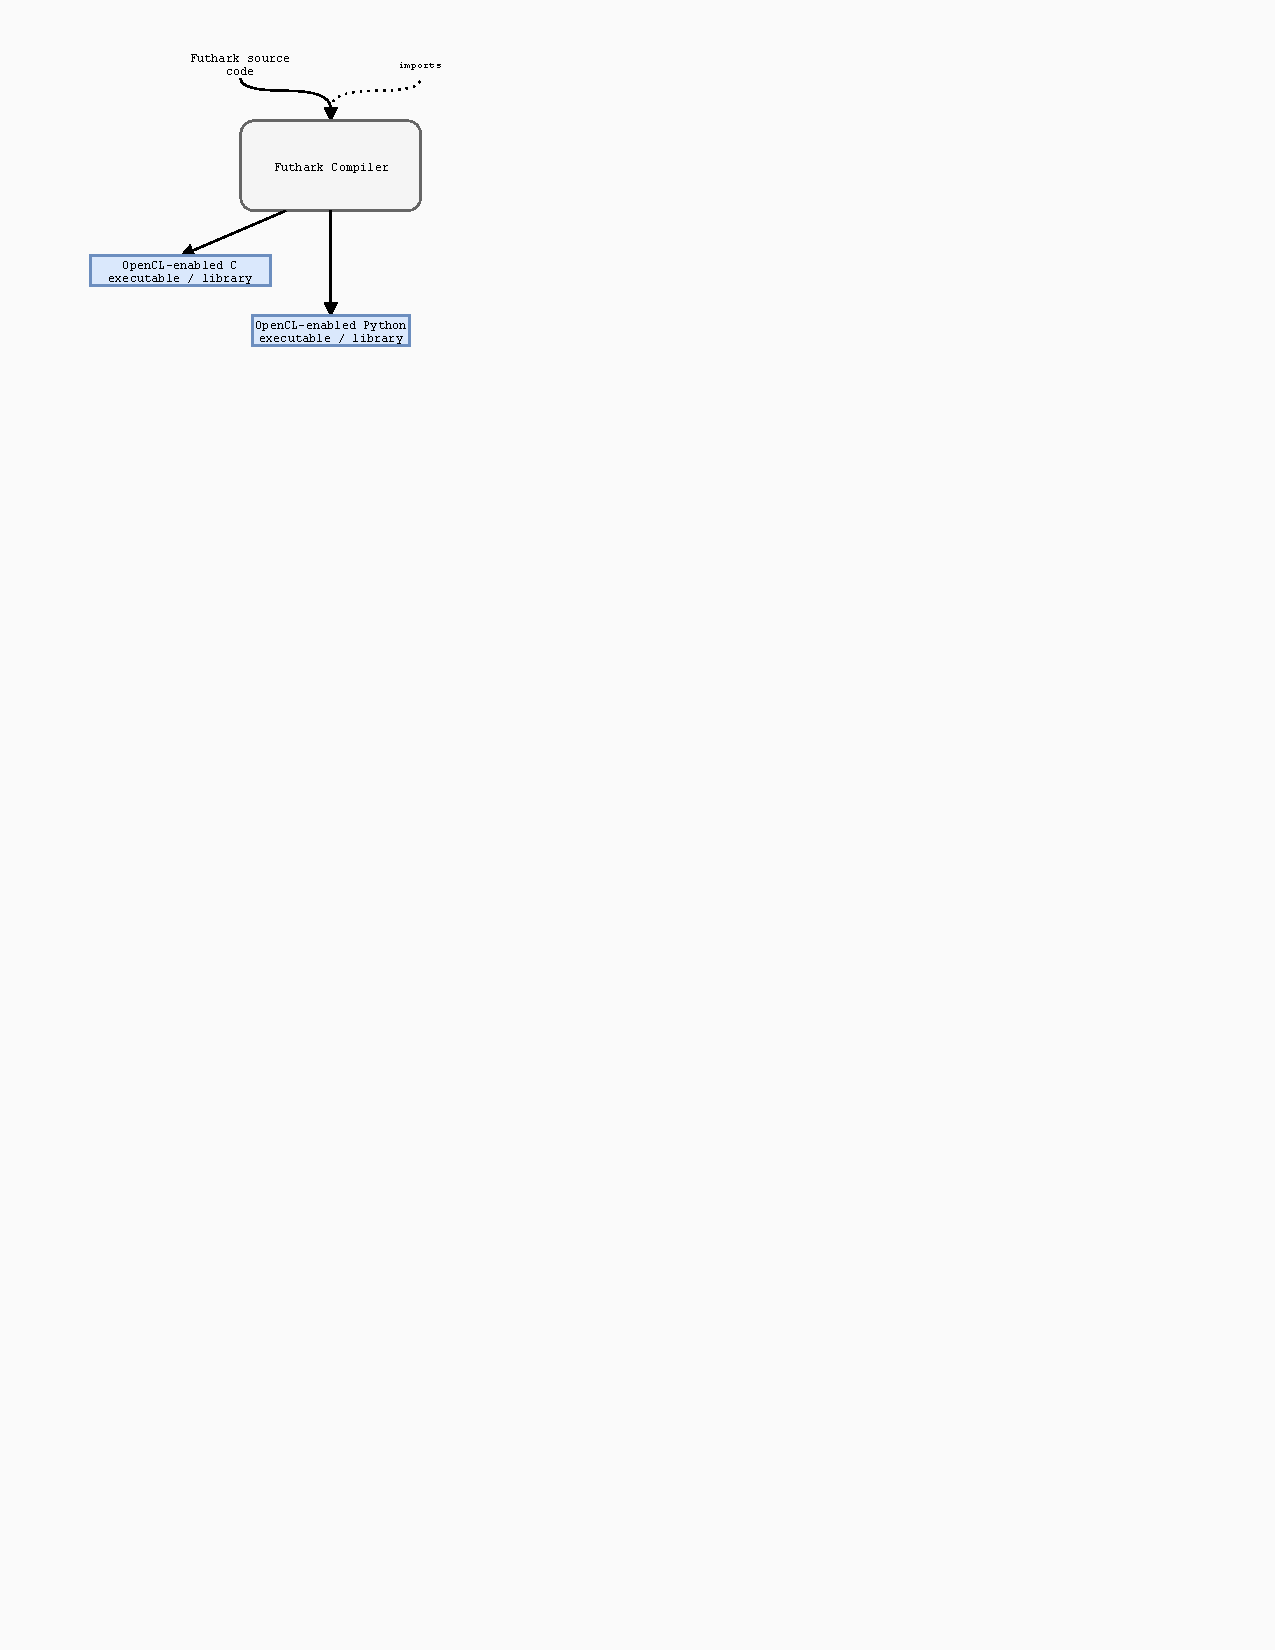
\includegraphics{./images/futhark_diagram_before.pdf}
        \onslide<2>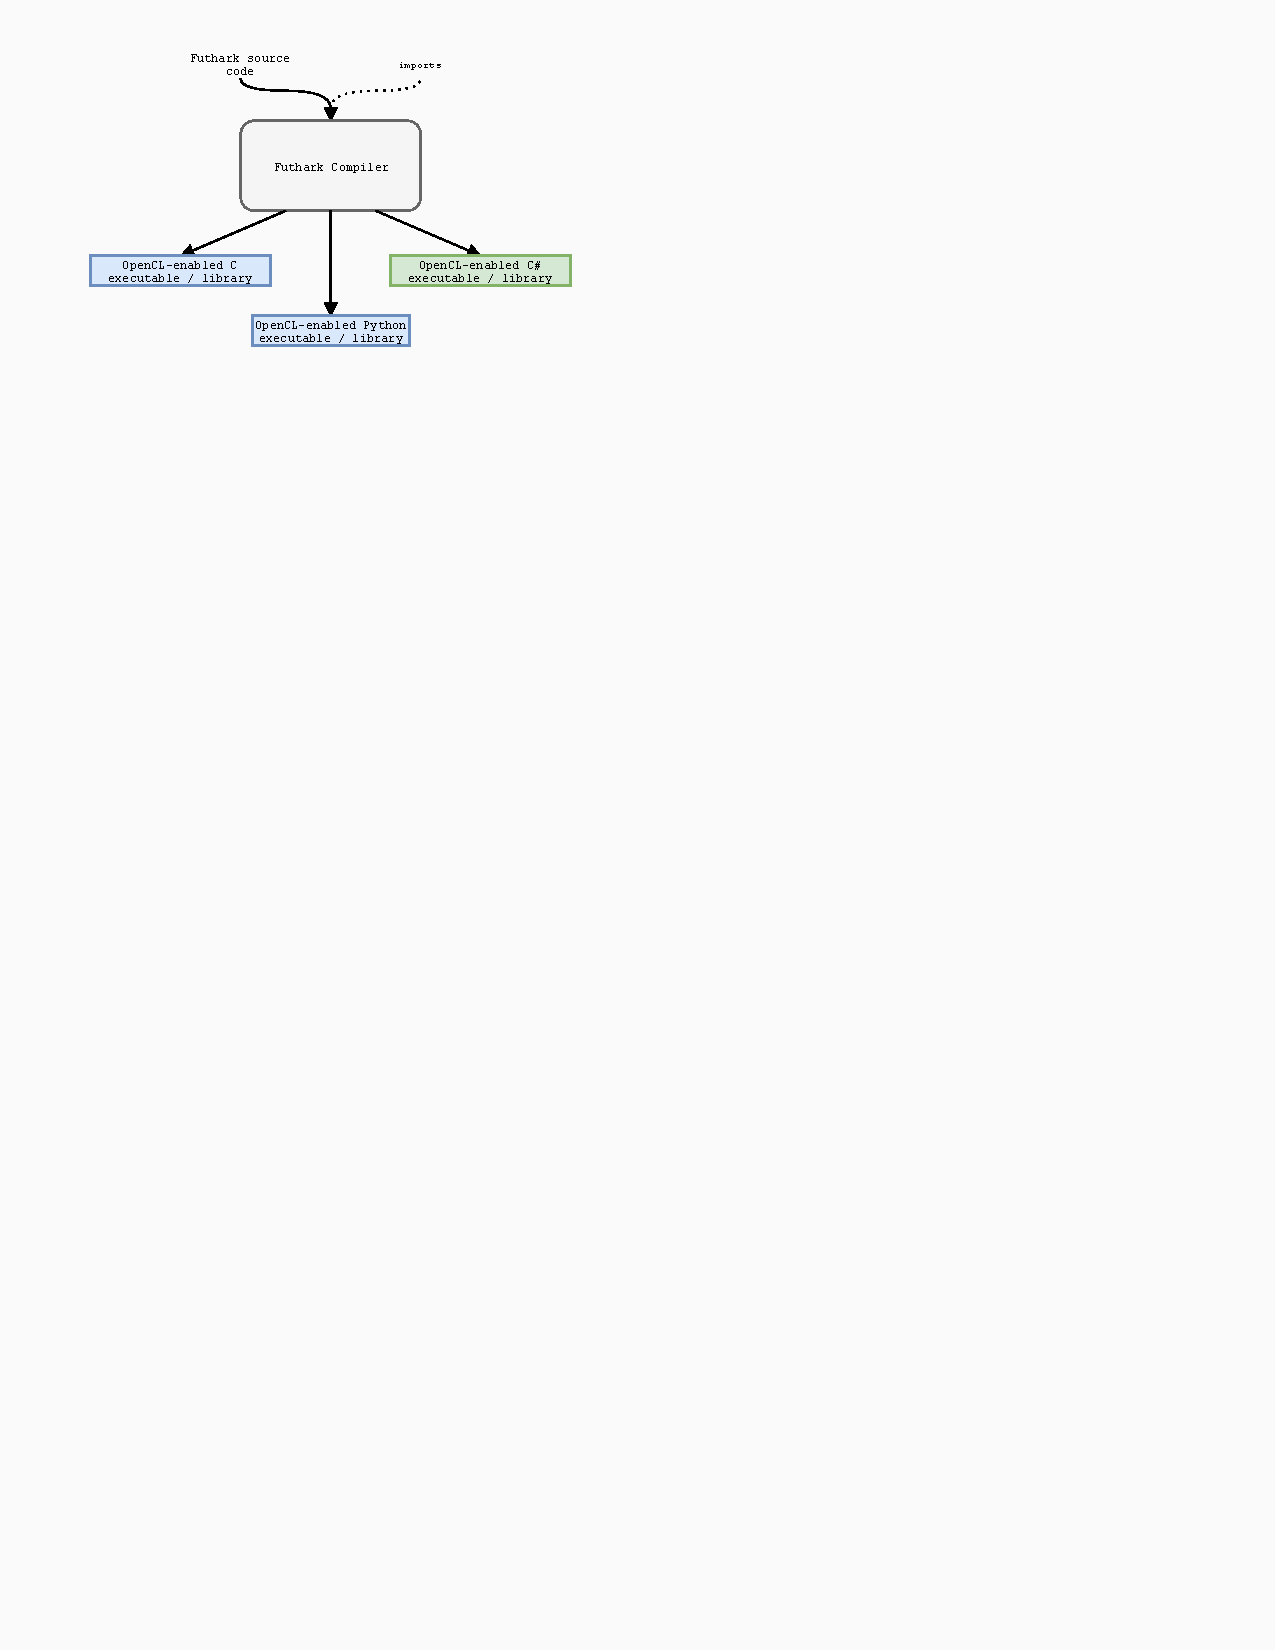
\includegraphics{./images/futhark_diagram_after.pdf}
      \end{overprint}
    \end{figure}

  %%% show diagram of futhark compilation pipeline
  %%%% for each part, elaborate and show example
\end{frame}

\begin{frame}[plain,c]
  \frametitle{Bird's eye view - The FShark Language}
  \begin{center}
    \Huge A language for GPU kernel programming
  \end{center}
\end{frame}

\begin{frame}[fragile, plain]
  \frametitle{Bird's eye view - The FShark Language}
\begin{columns}[T] % align columns
\begin{column}{.48\textwidth}
Prelude functions:\\
\begin{minted}[fontsize=\tiny, breaklines]{fsharp}
Replicate : int -> 't -> 't []

Iota : int -> int []

Transpose : 't [][] -> 't [][]

Map : (a -> b) -> a [] -> b []

Foldr : (a -> b -> b) -> b -> a [] -> b

Map2 : (a -> b -> c) -> a [] -> b [] -> c []
\end{minted}
\end{column}%
\hfill%
\pause
\begin{column}{.48\textwidth}
\texttt{matrix.fs}:
\begin{minted}[fontsize=\tiny, breaklines, linenos=true]{fsharp}
module Matrix
open FSharkPrelude
\end{minted}
\pause
\begin{minted}[fontsize=\tiny, breaklines, linenos=true, firstnumber=last]{fsharp}
type replicateRows : int -> int -> int [][] 
type multiply : int [][] 
                -> int [][] 
                -> int [][]
\end{minted}
\pause
\begin{minted}[fontsize=\tiny, breaklines, linenos=true, firstnumber=last]{fsharp}
let replicateRows n m = Replicate n [|1..m|]
\end{minted}
\pause
\begin{minted}[fontsize=\tiny, breaklines, linenos=true, firstnumber=last]{fsharp}
let multiply A B =
  let BT = Transpose B
\end{minted}
\pause
\begin{minted}[fontsize=\tiny, breaklines, linenos=true, firstnumber=last]{fsharp}
  let Sum = Foldr (+) 0
\end{minted}
\pause
\begin{minted}[fontsize=\tiny, breaklines, linenos=true, firstnumber=last]{fsharp}
  in Map (fun row ->
       Map (fun col -> 
         Sum <| Map2 (*) row col
       ) BT
     ) A
\end{minted}
\end{column}%
\end{columns}
\end{frame}

\begin{frame}[plain,c]
  \frametitle{Bird's eye view - The FShark Compiler/Wrapper}
  \begin{center}
    \Huge An FShark compilation/invokation pipeline
  \end{center}
\end{frame}

\begin{frame}[fragile]
  \frametitle{Bird's eye view - The FShark Compiler/Wrapper}
\begin{columns}[t] % align columns
\begin{column}{.38\textwidth}
\begin{minted}[fontsize=\tiny,linenos,breaklines, linenos=true]{fsharp}
module FSharkExample
open FShark.Main

let main argv =
  let wrapper = 
    new FSharkWrapper(
      libName="MatrixExample",
      tmpRoot="./",
      preludePath= "./FSharkPrelude.dll",
      openCL=true,
      unsafe=true,
      debug=false
      )
\end{minted}
\vfill
\end{column}
\pause
\hfill
\begin{column}{.60\textwidth}
  \begin{figure}
    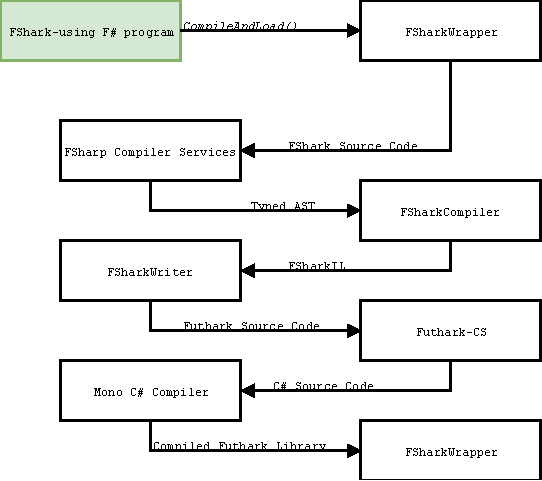
\includegraphics[scale=0.7]{./images/pipeline/pipeline1}
  \end{figure}
\end{column}
\end{columns}
\vfill
\end{frame}

\begin{frame}[fragile]
  \frametitle{Bird's eye view - The FShark Compiler/Wrapper}
\begin{columns}[t] % align columns
\begin{column}{.38\textwidth}
  \begin{figure}
\begin{minted}[fontsize=\tiny,linenos,breaklines, linenos=true]{fsharp}
module FSharkExample
open FShark.Main

let main argv =
  let wrapper = 
    new FSharkWrapper(
      libName="MatrixExample",
      tmpRoot="./",
      preludePath= "./FSharkPrelude.dll",
      openCL=true,
      unsafe=true,
      debug=false
      )
  wrapper.AddSourceFile "matrix.fs"
  wrapper.CompileAndLoad
\end{minted}
  \end{figure}
\end{column}
\hfill
\begin{column}{.60\textwidth}
  \begin{figure}
    \begin{overprint}
      \only<1>{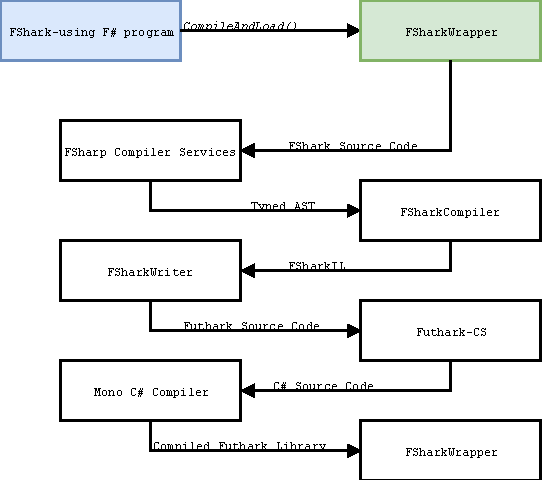
\includegraphics[scale=0.7]{./images/pipeline/pipeline2}}
      \only<2>{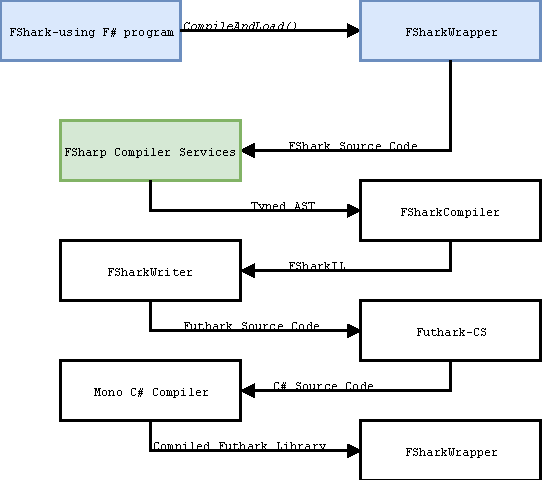
\includegraphics[scale=0.7]{./images/pipeline/pipeline3}}
      \only<3>{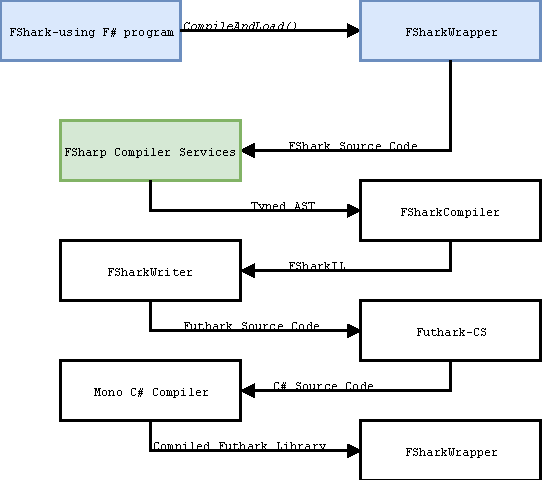
\includegraphics[scale=0.7]{./images/pipeline/pipeline4}}
    \end{overprint}
  \end{figure}
\end{column}
\end{columns}
\end{frame}
  %% fshark transpiler and wrapping framework
  %%% explain use case
  %%% show large diagram of components, and explain individual parts
  %%%% for each part, elaborate and show example
  
\begin{frame}[fragile]
  \frametitle{Bird's eye view - The FShark Compiler/Wrapper}
\begin{columns}[t] % align columns
\begin{column}{.38\textwidth}
  \begin{figure}
\begin{minted}[fontsize=\tiny, breaklines, linenos=true]{fsharp}
let multiply A B =
  let BT = Transpose B
  let Sum = Foldr (+) 0
  in Map (fun row ->
       Map (fun col -> 
         Sum <| Map2 (*) row col
       ) BT
     ) A
\end{minted}
  \end{figure}
\end{column}
\hfill
\begin{column}{.60\textwidth}
  \begin{figure}
    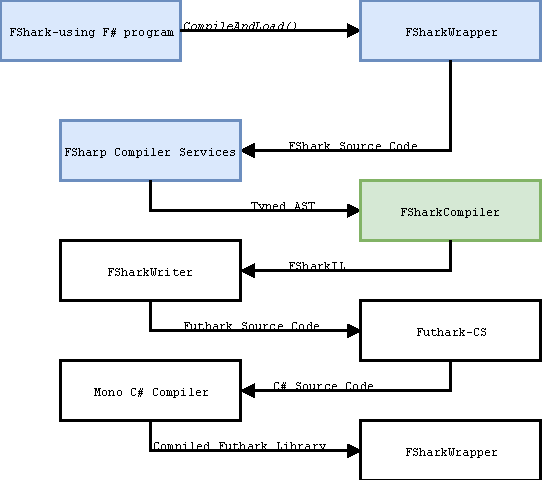
\includegraphics[scale=0.7]{./images/pipeline/pipeline5}
  \end{figure}
\end{column}
\end{columns}
\end{frame}

\begin{frame}[fragile]
  \frametitle{Bird's eye view - The FShark Compiler/Wrapper}
\begin{columns}[t] % align columns
\begin{column}{.38\textwidth}
  \begin{figure}
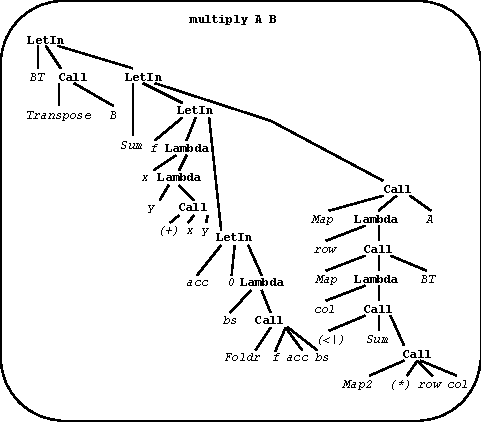
\includegraphics[scale=0.6]{./images/multiplyAST}
  \end{figure}
\end{column}
\hfill
\begin{column}{.60\textwidth}
  \begin{figure}
    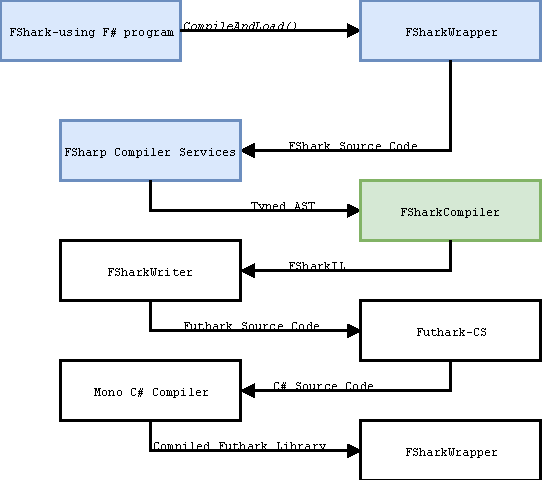
\includegraphics[scale=0.7]{./images/pipeline/pipeline5}
  \end{figure}
\end{column}
\end{columns}
\end{frame}

\begin{frame}[fragile]
  \frametitle{Bird's eye view - The FShark Compiler/Wrapper}
\begin{columns} % align columns
\begin{column}{.38\textwidth}
\begin{minted}[fontsize=\tiny,linenos,breaklines, linenos=true]{fsharp}
module FSharkExample
open FShark.Main

let main argv =
  let wrapper = 
    new FSharkWrapper(
      libName="MatrixExample",
      tmpRoot="./",
      preludePath= "./FSharkPrelude.dll",
      openCL=true,
      unsafe=true,
      debug=false
      )
  wrapper.AddSourceFile "matrix.fs"
  wrapper.CompileAndLoad
\end{minted}
\begin{minted}[fontsize=\tiny,linenos, linenos=true, firstnumber=last]{fsharp}
  let n = 5;
  let m = 7;
  let p = 6;

  let A =
    wrapper.InvokeFunction("replicateRows",n,m);
  let B = 
    wrapper.InvokeFunction("replicateRows",m,p);
  let AB = 
    wrapper.InvokeFunction("multiply",A,B);

  printfn "Multiplying A with B gives us %A" AB
  0
\end{minted}
\end{column}
\begin{column}{.60\textwidth}
  \begin{figure}
    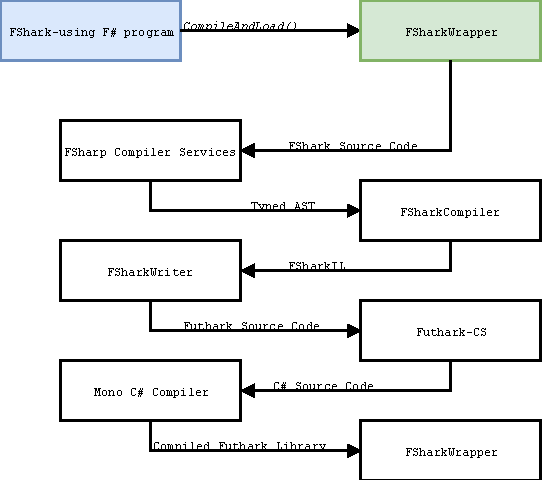
\includegraphics[scale=0.7]{./images/pipeline/pipeline2}
  \end{figure}
\end{column}
\end{columns}
\end{frame}

\begin{frame}[fragile]
  \frametitle{Bird's eye view - The FShark Compiler/Wrapper}
  % Choosing what types FShark should support, and how to implement the support
  % for these types. in particular the whole ding about arrays.

  % interoperability between F# and generated C# libraries
\end{frame}
\begin{frame}[fragile]
  \frametitle{Challenges}
  % Choosing what types FShark should support, and how to implement the support
  % for these types. in particular the whole ding about arrays.

  % interoperability between F# and generated C# libraries
\end{frame}

\begin{frame}[fragile]
  \frametitle{Challenges - Choosing an array type for FShark}
  \begin{itemize}
  \item <1-> Futhark is an array programming language
  \item <2-> FShark arrays need to sufficiently enable SOAC- and multidimensional
  \item <3-> F\# supports both jagged- and multidimensional arrays.
  \end{itemize}
  % Choosing what types FShark should support, and how to implement the support
  % for these types. in particular the whole ding about arrays.
\end{frame}
\begin{frame}[fragile]
  \frametitle{Challenges - Choosing an array type for FShark}
  \begin{itemize}
  \item <1-> Futhark is an array programming language
  \item <2-> FShark arrays need to sufficiently enable SOAC- and multidimensional
  \item <3-> F\# supports both jagged- and multidimensional arrays.
  \end{itemize}
  % Choosing what types FShark should support, and how to implement the support
  % for these types. in particular the whole ding about arrays.
\end{frame}

\begin{frame}[fragile,fragile]
  \frametitle{Challenges - Choosing an array type for FShark}
{\onslide<1->
  Multidimensional arrays:\\
}
{\onslide<2->
\begin{figure}
  \centering
  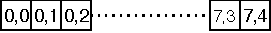
\includegraphics[scale=1]{./images/flatarrays}
\end{figure}
}

{\onslide<3->
  \texttt{let xs = array2D.init 8 5 (fun \_ \_ -> 0)}\\
  \texttt{let ys = array3D.init 8 5 5 (fun \_ \_ \_ -> 0)}
}
\end{frame}
\begin{frame}
  \frametitle{Challenges - Choosing an array type for FShark}
  Jagged arrays:\\
  \begin{columns}
    \begin{column}{.48\textwidth}
  \begin{figure}
    \centering
    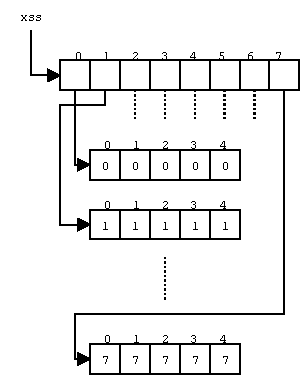
\includegraphics[scale=1]{./images/jaggedarrays}
  \end{figure}
    \end{column}
    \begin{column}{.48\textwidth}
    \end{column}
  \end{columns}
  % Choosing what types FShark should support, and how to implement the support
  % for these types. in particular the whole ding about arrays.
\end{frame}
\begin{frame}[fragile]
  \frametitle{Challenges - Choosing an array type for FShark}
  Jagged arrays:\\
  \begin{columns}
    \begin{column}{.48\textwidth}
  \begin{figure}
    \centering
    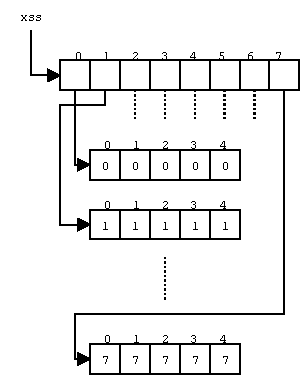
\includegraphics[scale=1]{./images/jaggedarrays}
  \end{figure}
    \end{column}
    \begin{column}{.48\textwidth}
\begin{minted}[fontsize=\scriptsize, breaklines]{fsharp}
let xs = [|
           [|0;0;0;0;0|];
           [|0;0;0;0;0|];
           ...
           [|0;0;0;0;0|];
         |] : int array array 

let ys = [|
           [|
             [|0;0;0;0;0|];
             [|0;0;0;0;0|];
             ...
             [|0;0;0;0;0|]
           |];
           ...
           [|
             [|0;0;0;0;0|];
             [|0;0;0;0;0|];
             ...
             [|0;0;0;0;0|]
           |];
         |] : int array array array
    \end{minted}
    \end{column}
  \end{columns}
  % Choosing what types FShark should support, and how to implement the support
  % for these types. in particular the whole ding about arrays.
\end{frame}
\begin{frame}[fragile]
  \frametitle{Challenges - Choosing an array type for FShark}
  Pros and cons:\\
  \begin{columns}
    \begin{column}{.48\textwidth}
      Multidimensional arrays:\\
      \begin{itemize}
      \item<1-> {\color{ForestGreen} \textbf{Flat memory layout}}
      \item<2-> {\color{ForestGreen} \textbf{Inherently regular arrays}}
      \item<3-> {\color{red} \textbf{Very limited SOAC support}}
      \end{itemize}
    \end{column}
    \begin{column}{.48\textwidth}
      Jagged arrays:\\
      \begin{itemize}
      \item<1-> {\color{red} \textbf{Scattered memory layout}}
      \item<2-> {\color{red} \textbf{No array layout guarantees*}} 
      \item<3-> {\color{ForestGreen} \textbf{Close-to-ideal SOAC support}}
      \end{itemize}
    \end{column}
  \end{columns}
  % Choosing what types FShark should support, and how to implement the support
  % for these types. in particular the whole ding about arrays.
\end{frame}

\begin{frame}[fragile]
  \frametitle{Challenges}
  % interoperability between F# and generated C# libraries
\end{frame}

\begin{frame}[fragile]
  \frametitle{Evaluation}
\end{frame}

\begin{frame}[fragile]
  \frametitle{Evaluation - Testing and correctness}
  How do we evaluate the individual parts of this thesis?
  \begin{itemize}
  \item<2-> C\# Code Generator:\\
    Evaluate using 960+ unit tests and 40+ benchmark programs.
  %% yes, based on unit tests and benchmark suite
\item<3-> The FShark Language:\\
  Write and use real life benchmark programs in FShark.
\item<4-> The FShark-to-Futhark translations:\\
  Evaluate using 128 unit tests.
  \end{itemize}
\end{frame}


\begin{frame}[fragile]
  \frametitle{Evaluation - Performance}
  % Look at how C# OpenCL performs compared to C OpenCL
  %% Boxplot for time increase/decrease for all benchmarks

  %% plot that describes runtime increase/decrease in correlation with input size

  %%% discuss where major differences comes from

  % Look at how C# performs compared to C
  %% Very few samples;
  %% Major differences
  %% Why are these differences so large?

  % All in all quite succesful
\end{frame}
\begin{frame}[fragile]
  \frametitle{Evaluation - Performance - Futhark benchmarks}
  
\end{frame}

\begin{frame}[fragile,c]
  \frametitle{Evaluation - Performance - FShark benchmarks}
  \begin{center}
  {\scriptsize
  \begin{tabular}{| l | l | c | c | r |}
    \hline			
    \textbf{Benchmark} & \textbf{Dataset} & \textbf{Futhark reference} & \textbf{FShark translation} & \textbf{Difference} \\
    \hline  
    Pathfinder & 100000 x 100 & 1062µ & 1092µ & +2.8\% \\
    \hline  
    Hotspot & 1024 x 1024 & 41779µ & 41630µ & -0.3\% \\
    \hline  
    Nbody & N = 100000 & 100085µ & 100072µ & -0.01\% \\
    \hline  
    LocVolCalib & medium.in & 132682µ & 263664µ & +99.5\% \\
    \hline  
  \end{tabular}
  }
    \end{center}
\end{frame}

\begin{frame}[fragile]
  \frametitle{Evaluation - Usability and interoperability}
  \begin{center}
    \Huge Live demo
  \end{center}
  
\end{frame}

\begin{frame}[fragile]
  \frametitle{Related work}
\end{frame}

\plain{Questions?}

\end{document}